% Method pipeline for the SID 2026 paper.
% Layout developed with an image model (paperbanana loop), then transcribed
% to TikZ so the labels are vector text at true IEEE sizes.
% Colours are style.py: GREEN chosen, RED abandoned, GREY context, ACCENT threshold.
\documentclass[border=2pt]{standalone}
\usepackage{times}
\usepackage{tikz}
\usetikzlibrary{arrows.meta}

\definecolor{pbgreen}{HTML}{2E7D5B}
\definecolor{pbred}{HTML}{B5484D}
\definecolor{pbink}{HTML}{2F2F2F}
\definecolor{pbgrey}{HTML}{E6E4DF}
\definecolor{pbcoast}{HTML}{B9B6B0}
\definecolor{pbaccent}{HTML}{3B6EA5}

\begin{document}
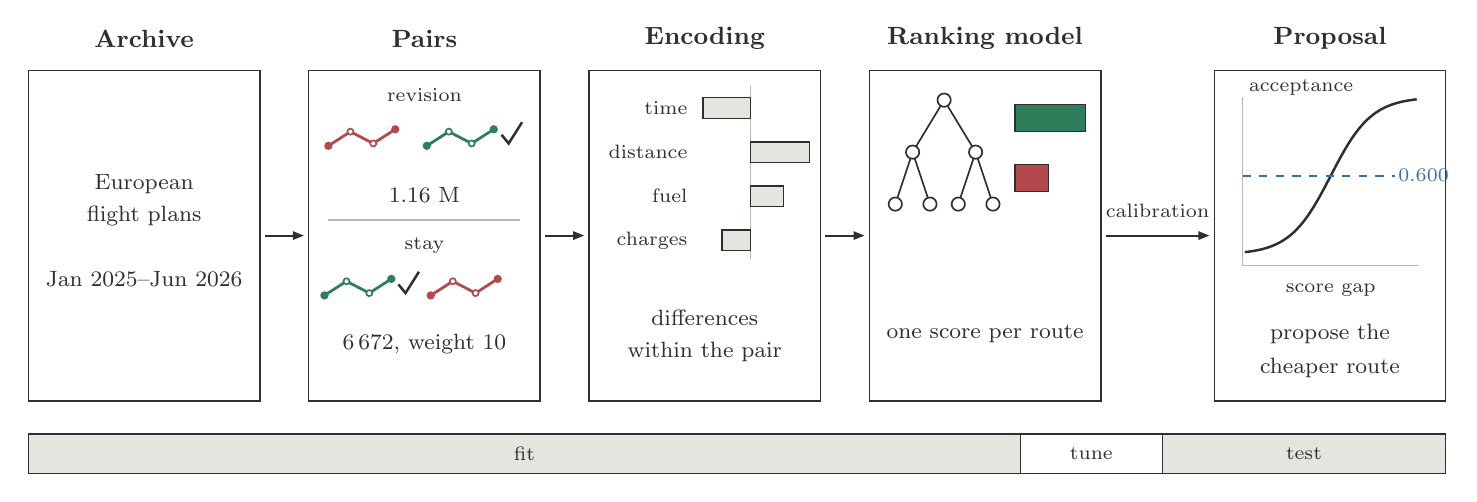
\begin{tikzpicture}[
  x=1cm, y=1cm,
  every node/.style={inner sep=0pt, outer sep=0pt, text=pbink},
  bx/.style={draw=pbink, line width=0.5pt, fill=white},
  flow/.style={draw=pbink, line width=0.7pt, -{Triangle[length=4pt,width=3pt]}},
  ttl/.style={font=\bfseries\small},
  txt/.style={font=\footnotesize},
  ann/.style={font=\scriptsize},
]

% Box origins. The last gap is wider so that "calibration" sits clear of both
% borders; every other gap is uniform.
\def\W{2.94}\def\H{4.2}\def\C{1.47}
\def\XA{0}\def\XB{3.56}\def\XC{7.12}\def\XD{10.68}\def\XE{15.06}

\foreach \x/\t in {\XA/Archive, \XB/Pairs, \XC/Encoding,
                   \XD/Ranking model, \XE/Proposal}{
  \draw[bx] (\x,0) rectangle (\x+\W,\H);
  \node[ttl] at (\x+\C,\H+0.40) {\t};
}
\foreach \a/\b in {\XA/\XB, \XB/\XC, \XC/\XD, \XD/\XE}{
  \draw[flow] (\a+\W+0.06,2.10) -- (\b-0.06,2.10);
}
\node[ann] at ({(\XD+\W+\XE)/2},2.42) {calibration};

% a route: two endpoint dots, two hollow waypoints, gentle dog-leg
\newcommand{\route}[3]{\begin{scope}[shift={(#2,#3)}]
  \draw[#1, line width=1.0pt]
    (0,0.10) -- (0.28,0.28) -- (0.57,0.13) -- (0.85,0.31);
  \fill[#1] (0,0.10) circle (1.5pt);
  \fill[#1] (0.85,0.31) circle (1.5pt);
  \draw[#1, line width=0.6pt, fill=white] (0.28,0.28) circle (1.1pt);
  \draw[#1, line width=0.6pt, fill=white] (0.57,0.13) circle (1.1pt);
\end{scope}}
\newcommand{\tick}[2]{\draw[pbink, line width=0.9pt]
  (#1,#2+0.08) -- (#1+0.09,#2-0.03) -- (#1+0.26,#2+0.24);}

% ---------- 1. archive ----------
\begin{scope}[shift={(\XA,0)}]
  \node[txt] at (\C,2.75) {European};
  \node[txt] at (\C,2.35) {flight plans};
  \node[txt] at (\C,1.55) {Jan 2025--Jun 2026};
\end{scope}

% ---------- 2. pairs ----------
\begin{scope}[shift={(\XB,0)}]
  \node[ann] at (\C,3.88) {revision};
  \route{pbred}{0.25}{3.14}   \route{pbgreen}{1.50}{3.14}
  \tick{2.45}{3.30}
  \node[txt] at (\C,2.62) {1.16 M};
  \draw[pbcoast, line width=0.5pt] (0.25,2.30) -- (2.69,2.30);
  \node[ann] at (\C,1.98) {stay};
  \route{pbgreen}{0.20}{1.24}
  \tick{1.14}{1.40}
  \route{pbred}{1.55}{1.24}
  \node[txt] at (\C,0.72) {6\,672, weight 10};
\end{scope}

% ---------- 3. encoding ----------
\begin{scope}[shift={(\XC,0)}]
  \draw[pbcoast, line width=0.5pt] (2.05,1.80) -- (2.05,4.00);
  \foreach \y/\lab/\dx in {3.72/time/-0.60, 3.16/distance/0.75,
                           2.60/fuel/0.42, 2.04/charges/-0.36}{
    \node[ann, anchor=east] at (1.25,\y) {\lab};
    \draw[bx, fill=pbgrey] (2.05,\y-0.13) rectangle (2.05+\dx,\y+0.13);
  }
  \node[txt] at (\C,1.05) {differences};
  \node[txt] at (\C,0.62) {within the pair};
\end{scope}

% ---------- 4. ranking model ----------
\begin{scope}[shift={(\XD,0)}]
  \coordinate (r) at (0.95,3.82);
  \coordinate (a) at (0.55,3.16);
  \coordinate (b) at (1.35,3.16);
  \draw[pbink, line width=0.6pt] (r) -- (a);
  \draw[pbink, line width=0.6pt] (r) -- (b);
  \foreach \p/\q in {a/0.33, a/0.77, b/1.13, b/1.57}{
    \draw[pbink, line width=0.6pt] (\p) -- (\q,2.50);
    \draw[pbink, line width=0.6pt, fill=white] (\q,2.50) circle (2.4pt);
  }
  \foreach \n in {r,a,b}{\draw[pbink, line width=0.6pt, fill=white] (\n) circle (2.4pt);}
  \draw[fill=pbgreen, draw=pbink, line width=0.4pt] (1.85,3.42) rectangle (2.75,3.76);
  \draw[fill=pbred,   draw=pbink, line width=0.4pt] (1.85,2.66) rectangle (2.28,3.00);
  \node[txt] at (\C,0.85) {one score per route};
\end{scope}

% ---------- 5. proposal ----------
\begin{scope}[shift={(\XE,0)}]
  \draw[pbcoast, line width=0.5pt] (0.36,1.72) -- (0.36,3.86);
  \draw[pbcoast, line width=0.5pt] (0.36,1.72) -- (2.60,1.72);
  \draw[pbink, line width=0.9pt, smooth, samples=60, domain=-4.2:4.2]
    plot ({1.48+\x*0.26}, {1.86+2.00/(1+exp(-\x))});
  \draw[pbaccent, line width=0.9pt, dashed] (0.36,2.86) -- (2.30,2.86);
  \node[ann, anchor=west, text=pbaccent] at (2.34,2.86) {0.600};
  \node[ann, anchor=west] at (0.44,3.98) {acceptance};
  \node[ann] at (1.48,1.40) {score gap};
  \node[txt] at (\C,0.85) {propose the};
  \node[txt] at (\C,0.42) {cheaper route};
\end{scope}

% ---------- split bar: 14 months, 1 month, 3 months ----------
\draw[bx, fill=pbgrey] (0,-0.92)     rectangle (12.60,-0.42);
\draw[bx, fill=white]  (12.60,-0.92) rectangle (14.40,-0.42);
\draw[bx, fill=pbgrey] (14.40,-0.92) rectangle (18.00,-0.42);
\node[ann] at (6.30,-0.67)  {fit};
\node[ann] at (13.50,-0.67) {tune};
\node[ann] at (16.20,-0.67) {test};

\end{tikzpicture}
\end{document}
